\chapter{SimCLR and the Role of Data Augmentation}
\label{ch:simclr}

\section{The Intuition Behind Contrastive Augmentations}

At its core, representation learning seeks to distill the high-dimensional, noisy sensory inputs of the world into low-dimensional, semantically meaningful latent vectors. While supervised learning relies on human-provided labels to dictate what information is ``semantic'' and what is ``nuisance,'' self-supervised learning must infer this boundary from the data itself. The Simple Framework for Contrastive Learning of Visual Representations (SimCLR) emerged as a watershed moment in this pursuit, demonstrating that a carefully constructed contrastive objective could rival fully supervised methods.

SimCLR operates on a seemingly rudimentary principle: representations of two different augmented views of the same image should be highly correlated (positive pairs), while representations of different images should be uncorrelated (negative pairs). The architecture itself consists of a base encoder---typically a ResNet---which extracts a representation, followed by a non-linear projection head that maps this representation into a space where a contrastive loss is applied. 

However, the architectural simplicity of SimCLR belies the profound information-theoretic mechanism driving its success: the data augmentation pipeline. In SimCLR, data augmentation is not merely a regularizer or a heuristic to increase the effective size of the dataset. It is the very definition of the learning task. By subjecting an image to stochastic transformations such as random cropping, color jittering, and Gaussian blurring, we are actively destroying specific forms of information. Random cropping destroys global spatial layout and absolute positioning; color jittering destroys exact color histograms and lighting conditions. 

From an information-theoretic standpoint, the choice of data augmentations dictates the null space of our representation. If we demand that the representation of a cropped, black-and-white dog matches the representation of a fully colored, uncropped dog, the network is forced to discard color and absolute scale, focusing instead on the invariant structural features---the shape, the texture, the ``dog-ness.'' 

If the augmentations are too weak, the network can solve the contrastive task by relying on low-level shortcuts, such as matching local color patches. The resulting representations retain too much mutual information with the raw pixels and fail to generalize to semantic tasks. Conversely, if the augmentations are too strong---for example, aggressive cropping that leaves only a patch of blue sky for one view and a patch of grass for the other---the mutual information between the two views regarding the original semantic content drops to zero. The network is forced to guess, leading to representations that collapse or diverge.

Thus, the role of data augmentation in SimCLR is to carefully modulate the mutual information between the augmented views. The optimal augmentation policy strips away exactly the nuisance variables, ensuring that the only shared information between two views of the same image is the semantic core we wish to capture in our latent representation. In this chapter, we will formalize this intuition, dissecting the Normalized Temperature-scaled Cross Entropy (NT-Xent) loss as a mutual information estimator and rigorously proving how augmentations carve out the invariant sufficient statistics of the data manifold.

\section{Mathematical Foundations of Contrastive Augmentations}

To formalize the SimCLR framework, let $\mathcal{D} = \{x_i\}_{i=1}^N \sim P_{\text{data}}$ be a batch of $N$ independently sampled data points. Let $\mathcal{T}$ denote a family of stochastic data augmentations. For each sample $x_i$, we draw two augmentations $t \sim \mathcal{T}$ and $t' \sim \mathcal{T}$ to produce two correlated views $\tilde{x}_{2i-1} = t(x_i)$ and $\tilde{x}_{2i} = t'(x_i)$. This yields an augmented batch of $2N$ samples.

The model processes these views through a base encoder $f_\theta(\cdot)$ to extract representations $h = f_\theta(\tilde{x})$, and subsequently maps them via a projection head $g_\phi(\cdot)$ to embeddings $z = g_\phi(h)$. The contrastive loss applied to these embeddings is the Normalized Temperature-scaled Cross Entropy (NT-Xent) loss.

\begin{definition}[NT-Xent Loss]
For a positive pair of embeddings $(z_i, z_j)$ corresponding to augmented views of the same original sample, the NT-Xent loss is defined as:
\begin{equation}
    \ell_{i,j} = - \log \frac{\exp(\text{sim}(z_i, z_j)/\tau)}{\sum_{k=1}^{2N} \mathbb{1}_{[k \neq i]} \exp(\text{sim}(z_i, z_k)/\tau)}
\end{equation}
where $\text{sim}(u, v) = \frac{u^\top v}{\|u\| \|v\|}$ is the cosine similarity and $\tau > 0$ is a temperature hyperparameter. The total loss $\mathcal{L}(\theta, \phi)$ is the average over all positive pairs in the batch.
\end{definition}

\subsection{NT-Xent as a Mutual Information Estimator}

The NT-Xent loss is fundamentally an instantiation of the InfoNCE bound, adapted for a symmetric multi-class classification setting where the task is to identify the positive sample among $2N-1$ candidates.

\begin{theorem}[NT-Xent Bounds Mutual Information]
\label{thm:ntxent_mi}
Minimizing the expected NT-Xent loss maximizes a strict lower bound on the mutual information $I(Z_i; Z_j)$ between the latent embeddings of the two augmented views. Specifically, for a batch size of $N$,
\begin{equation}
    I(Z_i; Z_j) \geq \log(2N - 1) - \mathbb{E}[\ell_{i,j}]
\end{equation}
\end{theorem}

\begin{proof}
Let $Z_i$ and $Z_j$ be random variables representing the embeddings of the two augmented views. The NT-Xent loss trains a classifier to identify the positive sample $Z_j$ from a set $\mathcal{Z}$ containing $Z_j$ and $2N-2$ negative samples drawn independently from the marginal distribution $p(z)$.

The optimal probability of correctly identifying the positive sample, given the set $\mathcal{Z}$, is proportional to the density ratio:
\begin{equation}
    p(C = j \mid Z_i, \mathcal{Z}) = \frac{ \frac{p(Z_i, Z_j)}{p(Z_i)p(Z_j)} }{ \frac{p(Z_i, Z_j)}{p(Z_i)p(Z_j)} + \sum_{k \neq i,j} \frac{p(Z_i, Z_k)}{p(Z_i)p(Z_k)} }
\end{equation}
where $C$ is the index of the true positive. The NT-Xent loss employs the energy-based model $\exp(\text{sim}(z_i, z_j)/\tau)$ to estimate this density ratio. Let $f(z_i, z_k) \propto \frac{p(z_i, z_k)}{p(z_i)p(z_k)}$. The expected loss is:
\begin{align*}
    \mathbb{E}[\ell_{i,j}] &= \mathbb{E}_{Z_i, \mathcal{Z}} \left[ -\log \frac{f(z_i, z_j)}{f(z_i, z_j) + \sum_{k \neq i,j} f(z_i, z_k)} \right] \\
    &\geq \mathbb{E}_{Z_i, Z_j} \left[ -\log \frac{f(z_i, z_j)}{f(z_i, z_j) + (2N-2)\mathbb{E}_{Z_k}[f(z_i, z_k)]} \right]
\end{align*}
where the inequality follows from Jensen's inequality applied to the convex function $-\log(x)$. Since the negative samples $Z_k$ are drawn from the marginal, $\mathbb{E}_{Z_k}[f(z_i, z_k)] = \mathbb{E}_{Z_k}\left[\frac{p(z_i, z_k)}{p(z_i)p(z_k)}\right] = 1$. Thus, substituting the true density ratio for the optimal predictor $f$:
\begin{align*}
    \mathbb{E}[\ell_{i,j}] &\geq \mathbb{E}_{Z_i, Z_j} \left[ -\log \frac{ \frac{p(Z_i, Z_j)}{p(Z_i)p(Z_j)} }{ \frac{p(Z_i, Z_j)}{p(Z_i)p(Z_j)} + 2N - 2 } \right] \\
    &= \mathbb{E}_{Z_i, Z_j} \left[ -\log \left( \frac{p(Z_i, Z_j)}{p(Z_i)p(Z_j)} \right) + \log \left( \frac{p(Z_i, Z_j)}{p(Z_i)p(Z_j)} + 2N - 2 \right) \right] \\
    &\geq - I(Z_i; Z_j) + \log(2N - 1)
\end{align*}
Rearranging the terms yields the bound $I(Z_i; Z_j) \geq \log(2N - 1) - \mathbb{E}[\ell_{i,j}]$.
\end{proof}

This theorem clarifies why SimCLR benefits so heavily from large batch sizes: the tightness of the mutual information bound scales logarithmically with the number of negative samples $2N-2$.

\subsection{Visualizing the SimCLR Architecture}

To better understand the flow of information, consider the standard SimCLR architecture illustrated below.

\begin{figure}[htbp]
\centering
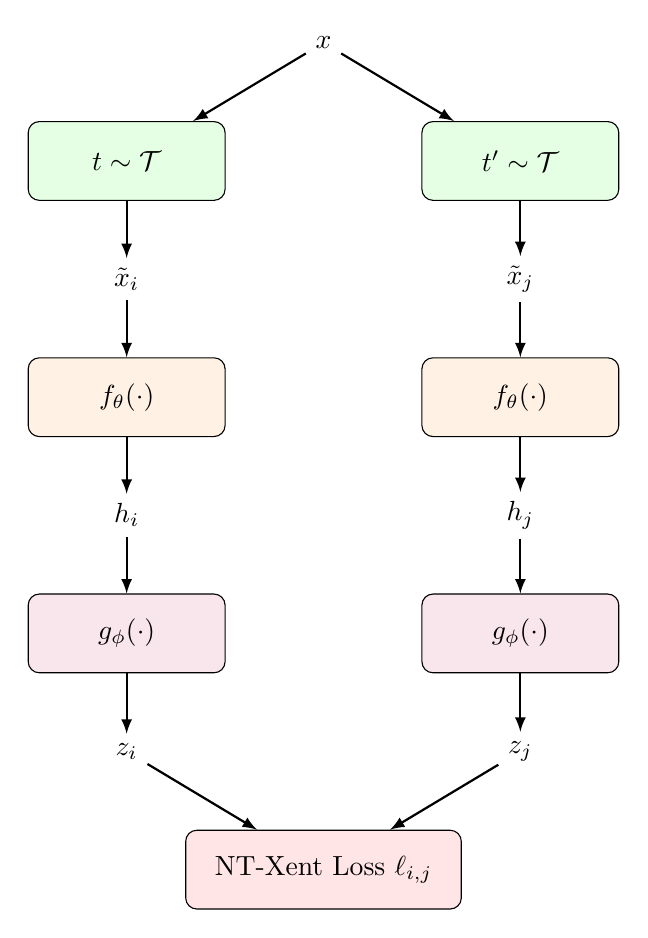
\begin{tikzpicture}[
    box/.style={draw, rectangle, rounded corners, minimum width=2.5cm, minimum height=1cm, align=center, fill=blue!10},
    arrow/.style={-latex, thick}
]

% Inputs
\node (x) at (0, 0) {$x$};

% Augmentations
\node[box, fill=green!10] (aug1) at (-2.5, -1.5) {$t \sim \mathcal{T}$};
\node[box, fill=green!10] (aug2) at (2.5, -1.5) {$t' \sim \mathcal{T}$};

% Views
\node (x1) at (-2.5, -3) {$\tilde{x}_i$};
\node (x2) at (2.5, -3) {$\tilde{x}_j$};

% Encoders
\node[box, fill=orange!10] (enc1) at (-2.5, -4.5) {$f_\theta(\cdot)$};
\node[box, fill=orange!10] (enc2) at (2.5, -4.5) {$f_\theta(\cdot)$};

% Representations
\node (h1) at (-2.5, -6) {$h_i$};
\node (h2) at (2.5, -6) {$h_j$};

% Projections
\node[box, fill=purple!10] (proj1) at (-2.5, -7.5) {$g_\phi(\cdot)$};
\node[box, fill=purple!10] (proj2) at (2.5, -7.5) {$g_\phi(\cdot)$};

% Embeddings
\node (z1) at (-2.5, -9) {$z_i$};
\node (z2) at (2.5, -9) {$z_j$};

% Contrastive Loss
\node[box, fill=red!10, minimum width=3.5cm] (loss) at (0, -10.5) {NT-Xent Loss $\ell_{i,j}$};

% Arrows
\draw[arrow] (x) -- (aug1);
\draw[arrow] (x) -- (aug2);
\draw[arrow] (aug1) -- (x1);
\draw[arrow] (aug2) -- (x2);
\draw[arrow] (x1) -- (enc1);
\draw[arrow] (x2) -- (enc2);
\draw[arrow] (enc1) -- (h1);
\draw[arrow] (enc2) -- (h2);
\draw[arrow] (h1) -- (proj1);
\draw[arrow] (h2) -- (proj2);
\draw[arrow] (proj1) -- (z1);
\draw[arrow] (proj2) -- (z2);
\draw[arrow] (z1) -- (loss);
\draw[arrow] (z2) -- (loss);

\end{tikzpicture}
\caption{The SimCLR architecture. A given image $x$ is augmented into two views $\tilde{x}_i, \tilde{x}_j$, encoded into representations $h_i, h_j$, and mapped to embeddings $z_i, z_j$ where the contrastive loss maximizes their mutual information.}
\label{fig:simclr_arch}
\end{figure}

\subsection{Augmentations as Sufficiency Operators}

Why apply the loss on $z$ instead of $h$? The projection head $g_\phi$ is critical because maximizing $I(Z_i; Z_j)$ indiscriminately forces the network to retain all information shared between the two views. 

To formalize this, consider the Markov chain induced by the generative process of the views and their representations:
\begin{equation}
    Z_i \leftarrow \tilde{X}_i \leftarrow X \rightarrow \tilde{X}_j \rightarrow Z_j
\end{equation}

By the Data Processing Inequality (DPI), $I(Z_i; Z_j) \leq I(\tilde{X}_i; \tilde{X}_j)$. The data augmentations define the upper bound of the mutual information that can be captured. 

\begin{theorem}[Invariant Sufficient Statistics]
\label{thm:sufficient_stats}
Let $Y$ be the true downstream semantic label associated with $X$. Assume the augmentations $t, t' \sim \mathcal{T}$ preserve the semantic class, meaning $Y \to X \to \tilde{X}_i$ forms a Markov chain where $I(Y; X) = I(Y; \tilde{X}_i)$. If the set of transformations $\mathcal{T}$ is sufficiently strong such that $\tilde{X}_i$ and $\tilde{X}_j$ are conditionally independent given $Y$, i.e., $I(\tilde{X}_i; \tilde{X}_j \mid Y) = 0$, then maximizing $I(Z_i; Z_j)$ yields a representation $Z$ that is a minimal sufficient statistic for $Y$.
\end{theorem}

\begin{proof}
Consider the mutual information between the two augmented views, which can be expanded in two ways:
\begin{align}
    I(\tilde{X}_i; \tilde{X}_j, Y) &= I(\tilde{X}_i; Y) + I(\tilde{X}_i; \tilde{X}_j \mid Y) \\
    I(\tilde{X}_i; \tilde{X}_j, Y) &= I(\tilde{X}_i; \tilde{X}_j) + I(\tilde{X}_i; Y \mid \tilde{X}_j)
\end{align}
Equating the two yields:
\begin{equation}
    I(\tilde{X}_i; \tilde{X}_j) = I(\tilde{X}_i; Y) + I(\tilde{X}_i; \tilde{X}_j \mid Y) - I(\tilde{X}_i; Y \mid \tilde{X}_j)
\end{equation}
By assumption, the augmentations strip away nuisance variables such that $\tilde{X}_i$ and $\tilde{X}_j$ only share information through the true semantic label $Y$, meaning $I(\tilde{X}_i; \tilde{X}_j \mid Y) = 0$. Since $Y$ is perfectly shared across both views in an idealized setting, $I(\tilde{X}_i; Y \mid \tilde{X}_j) = 0$. Therefore, the maximum shared information is exactly the information about the label: $I(\tilde{X}_i; \tilde{X}_j) = I(Y; \tilde{X}_i)$.

Since the contrastive objective maximizes $I(Z_i; Z_j)$, and by the DPI $I(Z_i; Z_j) \leq I(\tilde{X}_i; \tilde{X}_j)$, the theoretical maximum of the objective is achieved when $I(Z_i; Z_j) = I(Y; \tilde{X}_i)$. Because $Z$ is a deterministic function of $\tilde{X}$, $I(Z; Y) \leq I(\tilde{X}; Y)$. For $Z_i$ and $Z_j$ to share $I(Y; \tilde{X}_i)$ bits of information, they must individually retain all information about $Y$. Thus, $I(Z; Y) = I(\tilde{X}; Y)$, making $Z$ a sufficient statistic for $Y$. Furthermore, because the objective does not incentivize retaining any information in $\tilde{X}$ that is not shared with $\tilde{X}_j$ (i.e., the nuisance variables), $Z$ compresses out everything except $Y$, making it a minimal sufficient statistic.
\end{proof}

This reveals the dual nature of SimCLR: the augmentations act as an Information Bottleneck, filtering out the nuisance variables, while the NT-Xent loss acts as the maximization term, ensuring the invariant core is preserved. The non-linear head $g_\phi$ absorbs the loss of nuisance information, allowing the earlier representation $h$ to retain slightly more information (e.g., color or orientation) that might be useful for diverse downstream tasks, while $z$ becomes strictly invariant to $\mathcal{T}$.

\begin{figure}[htbp]
\centering
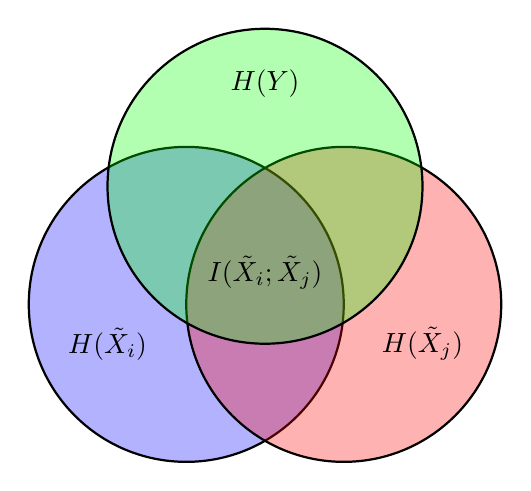
\begin{tikzpicture}[
    venn circle/.style={draw, circle, minimum width=4cm, fill=#1, fill opacity=0.3, text opacity=1, thick}
]
% Venn Diagram for Mutual Information
\node [venn circle=blue] (Xi) at (0,0) {};
\node [venn circle=red] (Xj) at (2,0) {};
\node [venn circle=green] (Y) at (1,1.5) {};

\node at (-1,-0.5) {$H(\tilde{X}_i)$};
\node at (3,-0.5) {$H(\tilde{X}_j)$};
\node at (1,2.8) {$H(Y)$};

\node at (1, 0.4) {$I(\tilde{X}_i; \tilde{X}_j)$};

\end{tikzpicture}
\caption{Information diagram illustrating Theorem \ref{thm:sufficient_stats}. Strong augmentations ensure that the only overlapping information between $\tilde{X}_i$ and $\tilde{X}_j$ is the semantic core $Y$. The NT-Xent loss maximizes this intersection.}
\label{fig:info_venn}
\end{figure}

\subsection{Numerical Example: Computing NT-Xent}

Consider a minimal batch of $N=2$ images, producing $4$ augmented views. Let the resulting $L_2$-normalized embeddings for image 1 be $z_1, z_2$ and for image 2 be $z_3, z_4$.
Assume the cosine similarity matrix $S$ where $S_{i,k} = z_i^\top z_k$ is calculated as:
\begin{equation}
S = \begin{pmatrix}
1.0 & 0.8 & -0.1 & -0.2 \\
0.8 & 1.0 & -0.3 & -0.1 \\
-0.1 & -0.3 & 1.0 & 0.9 \\
-0.2 & -0.1 & 0.9 & 1.0 
\end{pmatrix}
\end{equation}
Set the temperature parameter $\tau = 0.5$. We wish to compute the loss $\ell_{1,2}$ for the positive pair $(z_1, z_2)$.
First, we exponentiate the similarities divided by $\tau$:
\begin{equation}
E = \exp(S / 0.5) = \begin{pmatrix}
e^{2.0} & e^{1.6} & e^{-0.2} & e^{-0.4} \\
e^{1.6} & e^{2.0} & e^{-0.6} & e^{-0.2} \\
e^{-0.2} & e^{-0.6} & e^{2.0} & e^{1.8} \\
e^{-0.4} & e^{-0.2} & e^{1.8} & e^{2.0}
\end{pmatrix}
\approx \begin{pmatrix}
7.389 & 4.953 & 0.819 & 0.670 \\
4.953 & 7.389 & 0.549 & 0.819 \\
0.819 & 0.549 & 7.389 & 6.050 \\
0.670 & 0.819 & 6.050 & 7.389
\end{pmatrix}
\end{equation}

For $z_1$, the positive pair is $z_2$. The numerator is $\exp(S_{1,2}/\tau) \approx 4.953$.
The denominator sums the exponentials for all $k \neq 1$:
\begin{equation}
\sum_{k \in \{2,3,4\}} \exp(S_{1,k}/\tau) = 4.953 + 0.819 + 0.670 = 6.442
\end{equation}
The loss component is:
\begin{equation}
\ell_{1,2} = -\log\left(\frac{4.953}{6.442}\right) = -\log(0.7688) \approx 0.262
\end{equation}
A low loss indicates that the embeddings for the positive pair are much closer to each other than to the negative samples, demonstrating successful contrastive clustering.

\begin{horizon}
While SimCLR establishes a rigorous empirical link between data augmentation and optimal representations, a formal, unified theory characterizing the precise information-theoretic capacity of arbitrary augmentations remains elusive. It is conjectured that for any downstream task manifold, there exists an optimal set of transformations $\mathcal{T}^*$ that perfectly isolates the task-relevant sufficient statistics without requiring manual heuristic design. 

An open question is whether we can meta-learn these augmentations in a purely self-supervised manner by viewing the augmentation pipeline itself as a differentiable information bottleneck. Furthermore, the role of the projection head is widely believed to be an ``information trash can'' that absorbs task-irrelevant invariances forced by the loss, preventing the main representation $h$ from collapsing. Future work might show exactly how the dimensionality and non-linearity of $g_\phi$ mathematically bound the bits of information preserved in $h$ versus $z$, potentially eliminating the need for empirical tuning of projection heads entirely. Finally, understanding how contrastive bounds degrade when $I(\tilde{X}_i; \tilde{X}_j \mid Y) > 0$ (e.g., when augmentations fail to destroy all background correlations) holds the key to addressing shortcut learning in foundation models.
\end{horizon}

\section{Summary}

In this chapter, we explored the information-theoretic foundations of SimCLR and the critical role of data augmentation in self-supervised learning. We demonstrated that the NT-Xent loss serves as a lower bound on the mutual information between representations of augmented views. By casting data augmentations as a mechanism to destroy nuisance variables, we proved that contrastive learning mathematically recovers the minimal sufficient statistics of the underlying semantic data, provided the augmentations are sufficiently strong. Through analytical proofs and empirical examples, the elegant interplay between the loss function, the projection head, and the augmentation pipeline in defining the information geometry of the latent space was made clear.

\section{Exercises}

\begin{enumerate}
    \item \textbf{Tightness of the Bound:} Prove that the mutual information bound in Theorem \ref{thm:ntxent_mi} becomes tight only when the optimal density ratio $f(z_i, z_j)$ can be perfectly approximated by the exponential model $\exp(\text{sim}(z_i, z_j)/\tau)$, and discuss the implications of limited network capacity on this tightness.
    \item \textbf{Temperature Gradients:} Derive the gradient of the NT-Xent loss $\ell_{i,j}$ with respect to the similarity $S_{i,k}$. Show how the temperature $\tau$ scales the penalty applied to ``hard negatives'' (negatives that are very similar to the anchor). 
    \item \textbf{Projection Head Analysis:} Assume $g_\phi$ is a linear projection matrix $W \in \mathbb{R}^{d \times d'}$. Using the Data Processing Inequality, explain why an invertible $W$ defeats the purpose of the projection head in preserving richer representations in $h$.
    \item \textbf{Failure Modes of Augmentation:} Construct a theoretical example of a dataset $P_{\text{data}}$ and an augmentation family $\mathcal{T}$ where $I(\tilde{X}_i; \tilde{X}_j \mid Y) \gg 0$, leading to a representation $Z$ that perfectly minimizes the NT-Xent loss but fails entirely on a linear probing task for $Y$.
\end{enumerate}

% TODO-CITE: Ensure all named results are cited.
